\chapter{Сведения из теории нейронных сетей}

\section{Функции потерь и метрики}
\subsection{$F_1score$}
Данная функция является метрикой и выражается следующими формулами:

\begin{align*}
    precision &= \frac{TP}{TP + FP}, \: recall = \frac{TP}{TP + FN}, \: \text{где} \\
    &\begin{cases}
        TP = \: \text{true positive} \\
        FP = \: \text{false positive} \\
        FN = \: \text{false negative}
    \end{cases}, \: \text{а} \\
    F_1score &= 2 \cdot \frac{precision \cdot recall}{precision + recall} = \frac{TP}{TP + 0.5(FP + FN)}
\end{align*}

Как было отмечено выше, набор данных несбалансирован, а значит такие метрики, как,
например, точность (accuracy) не смогут описать достоверно качество
предсказания, однако с данной задачей хорошо справляется F-мера, благодаря чему
и была выбрана.

\subsection{Бинарная кроссэнтропия}

\subsection{DICE}

\section{Инструменты для улучшения качества предсказания и ускорения обучения}

\subsection{Пакетная нормализация}
Пакетная нормализация --- прием, заключающийся в добавлении некоторой операции
до и/или после функции активации каждого скрытого слоя. По сути она центрирует
возле нуля и нормализует каждый слой, затем масштабирует и сдвигает результат с
помощью двух новых векторов параметров на слой: один для сдвига, другой для
масштабирования. Другими словами, эта операция позволяет нейросети найти
оптимальные среднее и масштаб входов всех слоев.

Сам алгоритм пакетной нормализации:
\begin{align*}
    z^{(i)} &= \gamma \otimes \hat x^{(i)} + \beta, \text{где} \\
    \hat x^{(i)} = \frac{x^{(i)} - \mu_B}{\sqrt{\sigma^2_B + \xi}}, \qquad
    \mu_B &= \frac{1}{m_B} \sum\limits_{i = 1}^{m_B}x^{(i)}, \qquad
    \sigma_B^2 = \frac{1}{m_B} \sum\limits_{i = 1}^{m_B}(x^{(i)} - \mu_B)^2
\end{align*}

\begin{align*}
    z^{(i)} & \: \text{ --- результат операции: это отмасштабированная и сдвинутая версия входов} \\
    \gamma & \: \text{ --- выходной параметр --- масштаб для слоя} \\
    \otimes & \: \text{ --- поэлементное умножение векторов} \\
    \hat x^{(i)} & \: \text{ --- вектор отцентрированных и нормализованных входов для экземпляра} \: i \\
    \beta & \: \text{ --- выходной параметр --- сдвиг для слоя} \\
    \mu_B & \: \text{ --- вектор средних входа, посчитанных по всему пакету} \\
    \sigma_B & \: \text{ --- вектор стандартных отклонений входа, так же считается по всему пакету} \\
    x & \: \text{ --- вход} \\
    m_B & \: \text{ --- количество элементов в пакете} \\
    \xi & \: \text{ --- небольшое число для того, чтобы избежать деления на 0}
\end{align*}

\subsection{Исключение}
Dropout или прореживание зарекомендовал себя как эффективный и действенный
способ регуляризации нейросети \cite{dropout-is-good}. Суть метода состоит в
том, что на этапе обучения в каждом пакете с указанными вероятностями
зануляются некоторые входы, благодаря чему в конечном итоге обучается не одна
модель, а ансамбль, при этом, каждая его компонента обучается на своем наборе
данных. Таким образом, получается некая аппроксимация алгоритма бэггинга,
описание которого выходит за рамки данной работы (для дополнительной информации
см. \cite{goodfellow}).

\subsection{Сверточные слои}
Свёрточные слои \cite{goodfellow} позволяют получить устойчивость
предсказывающего алгоритма к локальным изменениям, таким как: сдвиг, поворот
или растяжение, а так же значительно снизить размеры входа, подаваемого
нейронной сети. Грубо говоря, данный слой выделяет паттерны на переданных ему
на вход данных. Эти слои находятся в самом начале нейронной сети и являются
кодировщиками, так как по сути на выходе они предоставляют нейросети некоторое
осмысленное представление входа.

\subsection{Остаточные связи}
Остаточные связи \cite{residual} --- это дополнительные связи между блоками
в нейронной сети (см. рис. \ref{fig:residual}). Данные связи помогают бороться с проблемой
затухающих градиентов, которая возникает в глубоких нейронных сетях из-за
специфики работы алгоритма обратного распространения ошибки, используемого для
обучения нейросети.

\begin{figure}[!htb]
    \centering
    \caption{Пример остаточной связи. F --- функция активации, x --- вход.}
    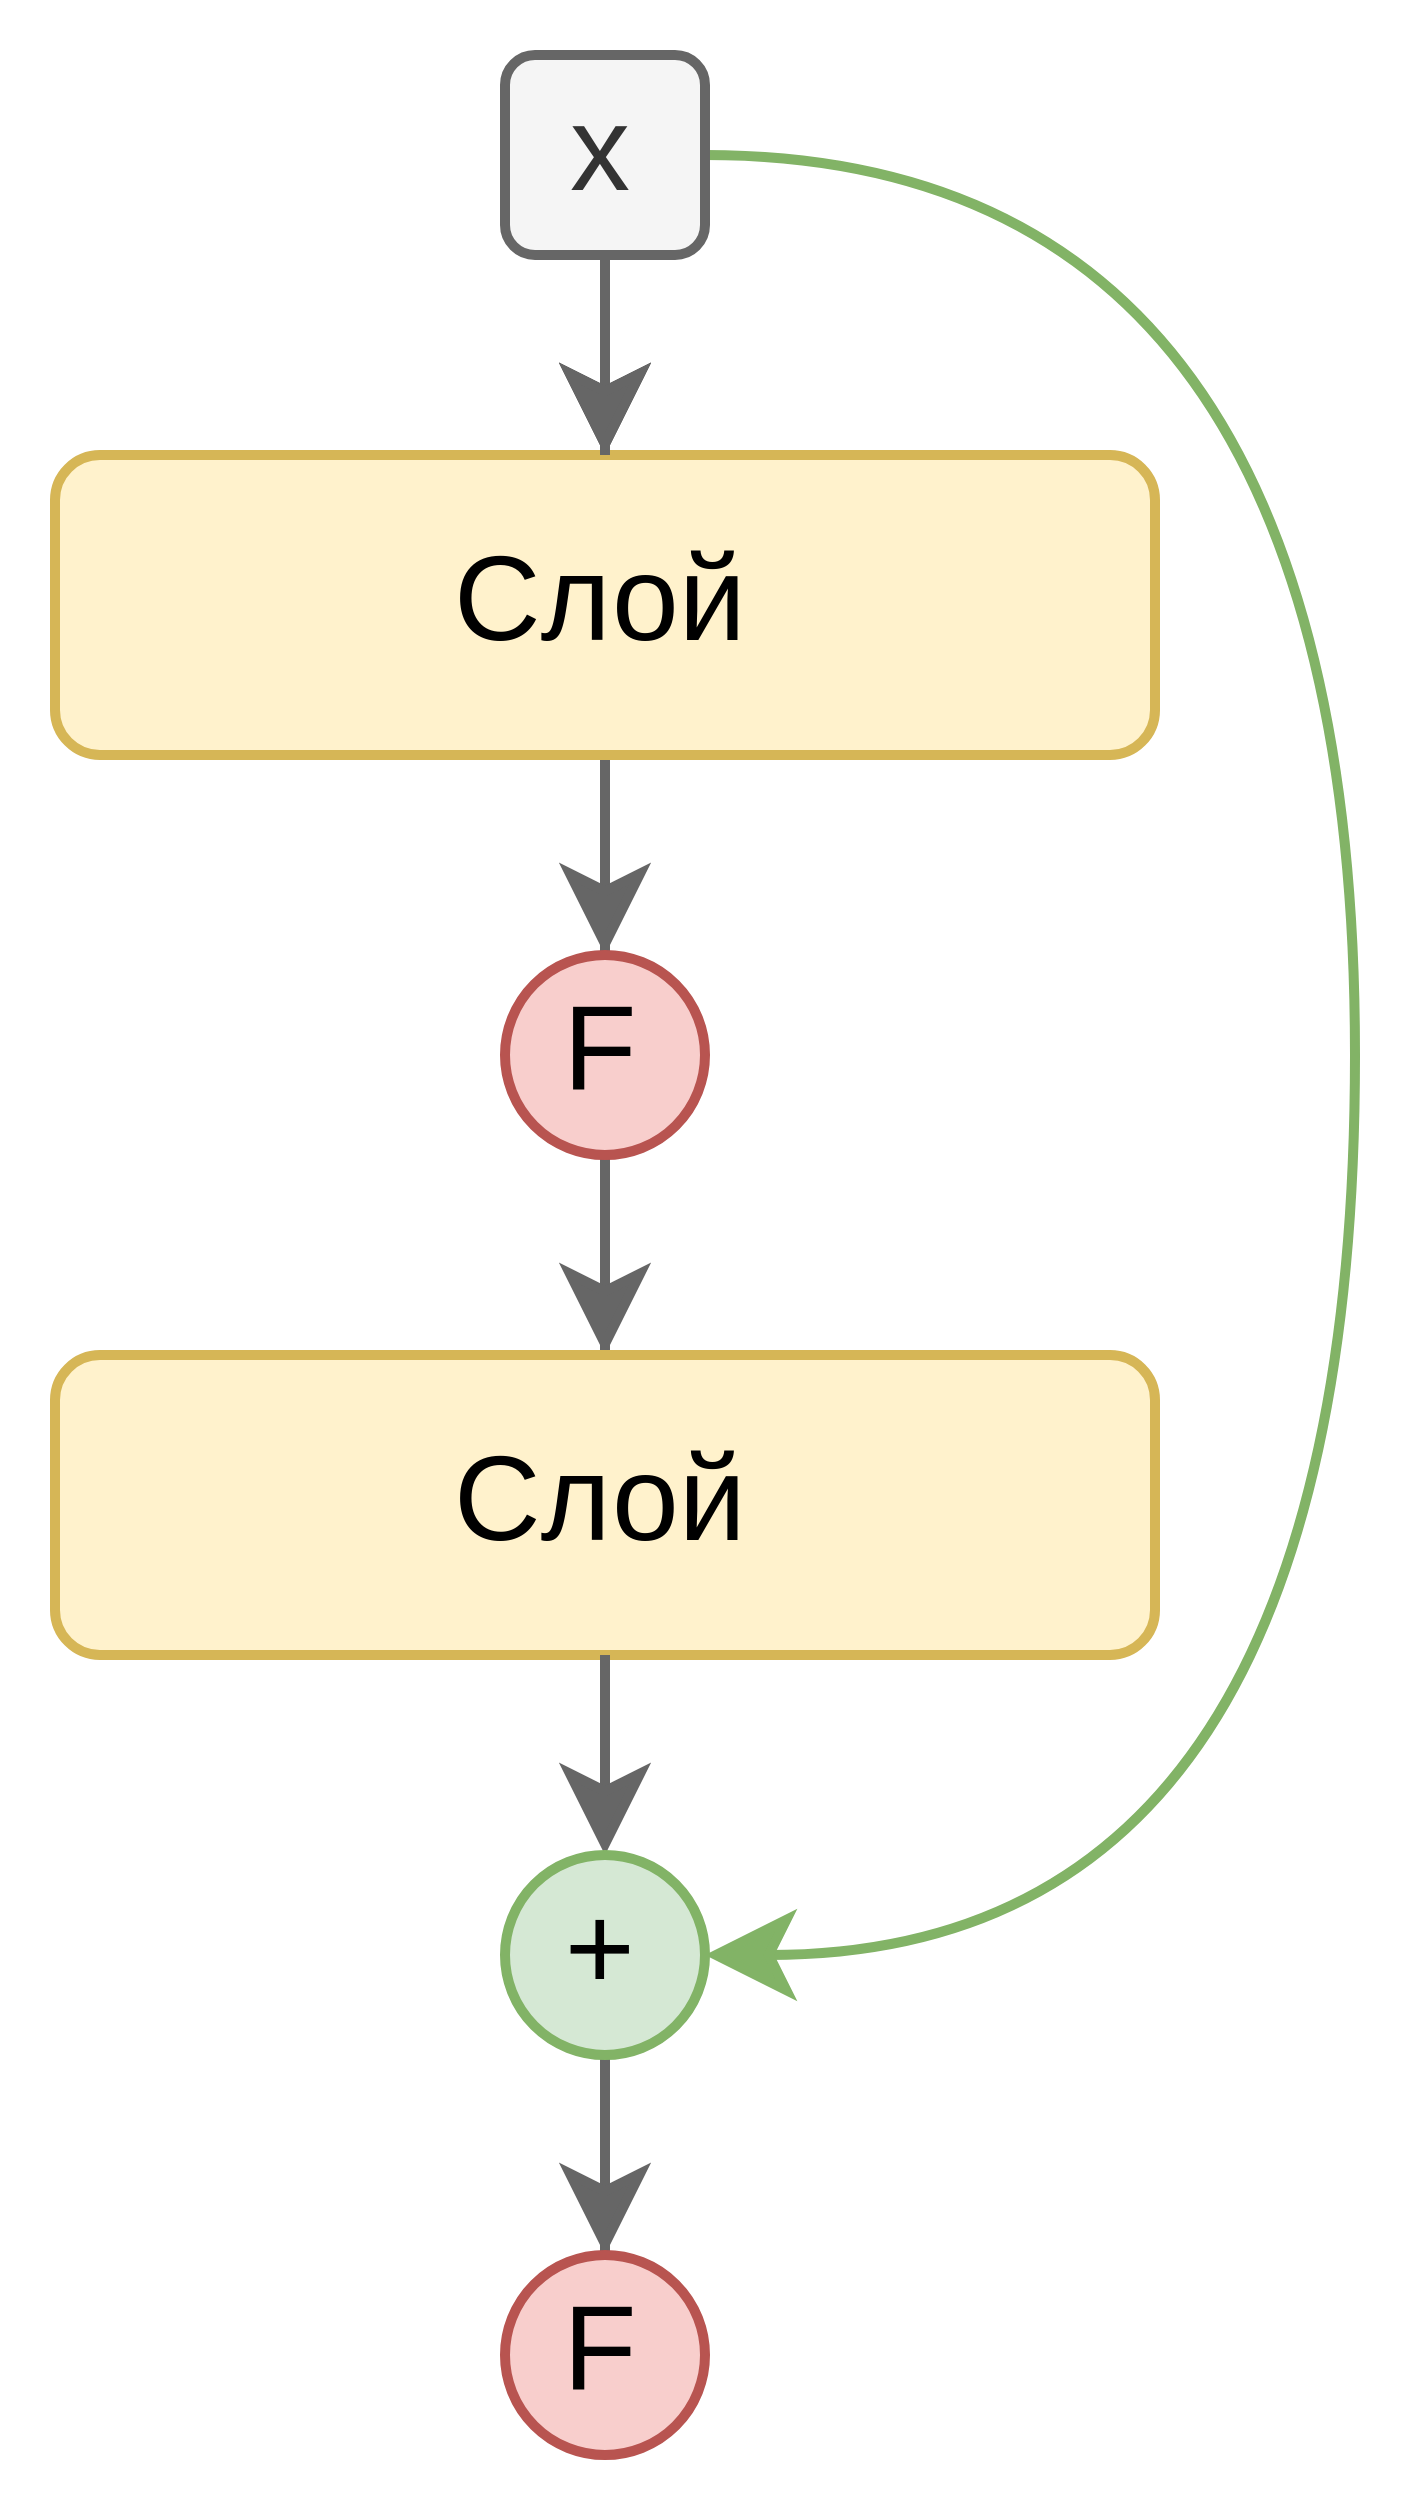
\includegraphics[width=0.25\textwidth]{residual}
    \label{fig:residual}
\end{figure}
